\documentclass[10pt]{beamer}

\usetheme[progressbar=frametitle]{metropolis}
\usepackage{appendixnumberbeamer}

\usepackage{booktabs}
\usepackage[scale=2]{ccicons}

\usepackage{pgfplots}
\usepgfplotslibrary{dateplot}

\usepackage{xspace}
\newcommand{\themename}{\textbf{\textsc{metropolis}}\xspace}

\title{Boston Airbnb Pricing}
\subtitle{An investigation using machine learning}
% \date{\today}
\date{}
\author{Group 7: Abhay Kasturia, Nakul Camasamudram, Philip Parker}
\institute{Northeastern University}
% \titlegraphic{\hfill\includegraphics[height=1.5cm]{logo.pdf}}

\begin{document}

\maketitle

\begin{frame}{Content}
  \setbeamertemplate{section in toc}[sections numbered]
  \tableofcontents[hideallsubsections]
\end{frame}


\section{Introduction}
	% ======================================================================
	\begin{frame}{Background Information}
    	\textbf{\textsc{Background:}}
    	\begin{itemize}
            \item Airbnb is a popular online company where property owners (known as ``hosts") can short-term rent their spaces
            \item A host must decide what daily price to charge for his or her space
            \item With data, this is clearly a supervised ML problem
            \item Issue: many real estate datasets include categorical location features with large numbers of levels
        \end{itemize}
        
        With this in mind, in this project we investigate two questions:
    \end{frame}
    
    % ======================================================================
    \begin{frame}{Questions to Investigate}
    	\begin{enumerate}
            \item To what degree can supervised machine learning techniques be used to assist an Airbnb host in determining an appropriate listing price for their property?
            \item For Airbnb data, can the categorical feature of ``neighborhood" be replaced with a continuous feature of driving distance to a geographic point of interest (e.g., an airport) and have comparable results?
        \end{enumerate}
    \end{frame}

\section{Methodology}
	% ======================================================================
	\begin{frame}{Data Collection and Preprocessing}
    	\textbf{\textsc{Data Source:}} Inside Airbnb Project - 4870 rows, 96 columns 
    	
        \textbf{\textsc{Features Selected:}}
        \fontsize{6pt}{7.2}\selectfont
    	\begin{columns}[T,onlytextwidth]
          \column{0.33\textwidth}
            \begin{itemize}
              	\item host\_is\_superhost
              	\item host\_identity\_verified
              	\item neighborhood
              	\item property\_type
              	\item room\_type
                \item accommodates
            \end{itemize}

          \column{0.33\textwidth}
          	\begin{itemize}
           		\item bathrooms
                \item bedrooms
                \item beds
                \item bed\_type
                \item guests\_included
                \item minimum\_nights
            \end{itemize}

          \column{0.33\textwidth}
            \begin{itemize}
              \item number\_of\_reviews
              \item instant\_bookable
              \item is\_business\_travel\_ready
              \item cancellation\_policy
              \item price
            \end{itemize}
        \end{columns}
        
        \fontsize{10pt}{7.2}\selectfont
        \textbf{\textsc{Outliers:}} 240 rows removed above the 95th percentile for price
        
        \textbf{\textsc{Missing Values:}} 14 rows  with missing values removed
    \end{frame}
    
    % ======================================================================
    \begin{frame}{Data Transformations and Partitions}
    	\textbf{\textsc{Transformations:}} Neighborhood feature replaced with distance to BOS Airport, to Downtown Crossing, and both
        
       	\textbf{\textsc{Partitions:}} Data partitioned into training, model selection, and two validation sets
        
        \begin{figure}[H]
        	\centering
        	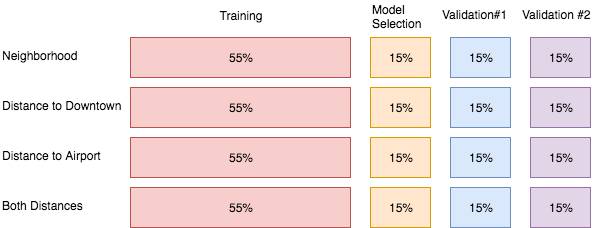
\includegraphics[width=\textwidth]{data_separation.png}
        \end{figure}
      \end{frame}
    
    % ======================================================================
    \begin{frame}{Applying Methods}
    	\textbf{\textsc{Methods Chosen:}} Linear Regression, GAMs, and Regression Trees
        \begin{itemize}
          \item For each method, we apply it to the different transformations in order to compare the effect of replacing the ``neighborhood" feature
          \item Afterward, we take the best transformation/method combination, and predict using the second validation set for a quality assessment of performance
        \end{itemize}  
    \end{frame}
    
    % ======================================================================
    \begin{frame}{Linear Regression}
    	\textbf{\textsc{Models:}} All predictors, Subset Selection, Lasso, Ridge
    
        \textbf{\textsc{Best:}} Lasso with $\lambda = 0.1135332$ and 58 predictors
        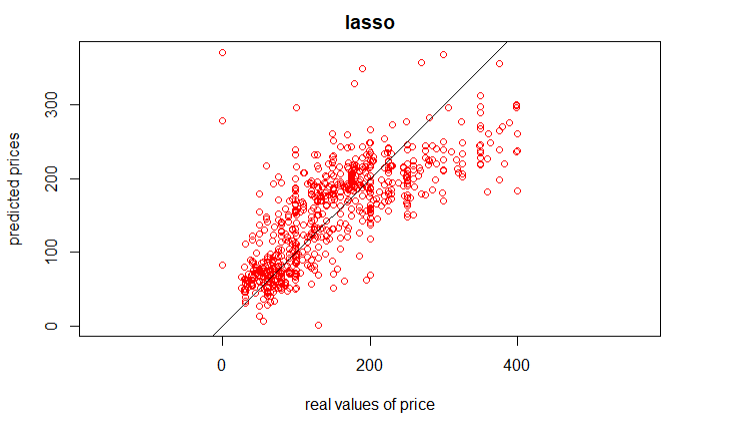
\includegraphics[width=\textwidth]{lasso.PNG}
    \end{frame}
    
    % ======================================================================
	\begin{frame}{Generalized Additive Models}
		\textbf{\textsc{Setup:}} Cubic splines for continuous features
    
        \textbf{\textsc{Term selection:}}
        	\begin{itemize}
        		\item Regression Subset Selection
                \item Forward Selection
                \item \textbf{Smoothness penalties with additional shrinkage term}
        	\end{itemize}
    \end{frame}
    
    % ======================================================================
    \begin{frame}{Regression Trees}
    	\textbf{\textsc{Considerations:}}
        \begin{itemize}
          \item Boosting used, as the importance of interpretability is small for our questions
          \item Cross-validation used to select number of trees = 10,000 
        \end{itemize} 
    	
    \end{frame}
    

\section{Results}
	% ======================================================================
	\begin{frame}{Most Important Predictors}
    	\textbf{\textsc{Linear Regression:}} neighborhood.South.End, neighborhood.Downtown, neighborhood.Beacon.Hill, neighborhood.Back.Bay, room\_type.Shared.room, room\_type.Private.room, property\_type.Other, bedrooms, accommodates~\\
        \textbf{\textsc{GAMs:}} neighborhood, property\_type, room\_type, instant\_bookable, accommodates, bedrooms, guests\_included ~\\
        \textbf{\textsc{Regression Trees:}}
        \begin{table}[H]
\centering

\label{my-label2}
\resizebox{\textwidth}{!}{
\begin{tabular}{l|ll|ll|ll|ll}
       & NVar & NRel & DDVar & DDRel & DAVar & DARel & DBVar    & DBRel \\ \hline
First  & room\_type       & 46.9             & room\_type    & 50.6          & room\_type   & 51.7         & room\_type   & 50.1      \\
Second & neighborhood     & 20.3             & bedrooms      & 15.7          & dairport     & 15.7         & bedrooms     & 15.8      \\
Third  & bedrooms         & 15.7             & ddowntown     & 15.1          & bedrooms     & 15.1         & ddowntown    & 11.5         
\end{tabular}}
\end{table}
    \end{frame}

	% ======================================================================
	\begin{frame}{Final Results}
    	\textbf{\textsc{Method/Transformation Comparison:}}
    	\begin{table}[H]
              \centering
              \label{my-label}
              \begin{tabular}{l|llll}
                                     & Linear Regression & GAM & Regression Trees &  \\ \cline{1-4}
                Neighborhood         & 56.82             &  55.15   &    55.75     &  \\
                Distance to Downtown & 58.95             &  58.05   &    57.00   &  \\
                Distance to Airport  & 60.76             &  56.24   &    56.57   &  \\
                Both Distances       & 58.16             &  55.77   &    56.54     & 
              \end{tabular}
            \end{table}
            
        \textbf{\textsc{Best Method/Transformation Performance:}} \\
        GAM on the original dataset with MSE = 52.30
        
    \end{frame}
    


\section{Discussion}
	% ======================================================================
	\begin{frame}{Question 1: Performance Useful?}
    	\textbf{\textsc{Question:}} To what extent can supervised ML techniques be used to assist a host in determining listing price?
        
        \textbf{\textsc{Answer:}} Useful, but information outside of these features is important.
        
    \end{frame}
    
    % ======================================================================
    \begin{frame}{Question 2: Transformations Reasonable?}
    	\textbf{\textsc{Question:}} For Airbnb data, can the ``neighborhood" feature be replaced with distance to a geographic point of interest?
        
        \textbf{\textsc{Answer:}} Yes.
        
    \end{frame}
    
    % ======================================================================
    \begin{frame}{Potential Improvements}
    	\begin{itemize}
          \item More sophisticated selection of POI
          \item Try to access information contained in textual data (e.g., sentiment analysis in reviews)
        \end{itemize}
        
    \end{frame}
    
        
    % ======================================================================
    \begin{frame}{Visualizations}
    	\textbf{\textsc{Listing price distribution across Boston (Darker = Expensive)}}
    	 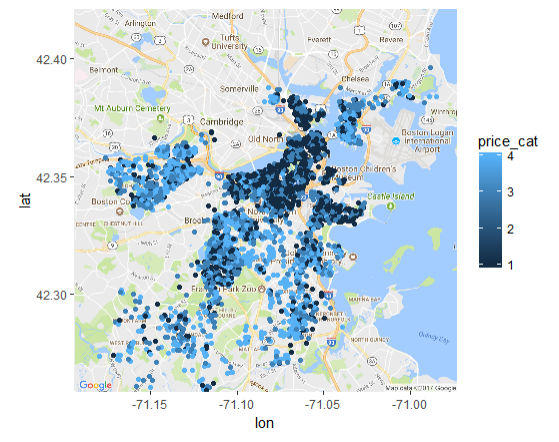
\includegraphics[width=\textwidth,scale=.7]{price_map.PNG} \\
    \end{frame}
    
    % ======================================================================
    \begin{frame}{Audience Questions}
    	\textbf{\textsc{Questions?}} 
        
    \end{frame}



\end{document}
